%!TEX root = ../../csuthesis\_main.tex
\chapter{实验流程}

\section{ChatScene 框架设计}

场景生成流程

固定场景模式:基于 Scenic 语言构建 8 类基准场景,涵盖城市道路、高速路、交叉路口等典型交通环境。采用深度强化学习中的软演员 - 评论家(SAC)算法,以碰撞避免、车道保持等作为奖励函数,优化对抗行为参数,模拟复杂交通参与者交互行为,为自动驾驶系统提供标准化测试场景。​
动态模式:接收用户自然语言描述,通过 API 调用 GPT-4o 模型,利用其强大的自然语言理解与代码生成能力,将自然语言转化为符合 CARLA 0.9.13 规范的场景代码。通过设定约束条件,如道路类型、车辆类型、交通规则等,生成多样化、贴近真实驾驶场景的测试用例。


关键模块

环境配置:以 CARLA 0.9.13 作为仿真核心,运行于 Ubuntu 系统环境。借助 TurboVNC 实现远程可视化,支持研究人员在不同终端实时观测场景运行状态。同时,利用 NVIDIA GPU 加速渲染,确保高分辨率、高帧率的场景渲染效果,提升仿真的真实性与流畅性 。​
对抗代理控制:Scenic 负责管理周围车辆的行为逻辑,通过预定义的规则与策略,模拟不同驾驶风格的交通参与者。RL 模型则专门控制自我车辆,通过与环境的交互学习,优化驾驶决策,在对抗性场景中实现安全、高效的驾驶行为。

\subsection{流程}
场景选择训练(train\_scenario模式)使用run\_train.py脚本调用场景优化流程。以脚本示例命令为例:

python scripts/run\_train.py --agent\_cfg=adv\_scenic.yaml --scenario\_cfg=train\_scenario\_scenic.yaml --mode train\_scenario --scenario\_id 1

其中adv\_scenic.yaml为智能体配置文件,train\_scenario\_scenic.yaml为场景配置文件,可指定样本数量(sample\_num)、优化步长(opt\_step)等参数。该步骤将从预定义场景和行为集中采样多个场景,并根据碰撞等指标选出最具挑战性的场景。

\begin{figure}[htbp]
	\centering
	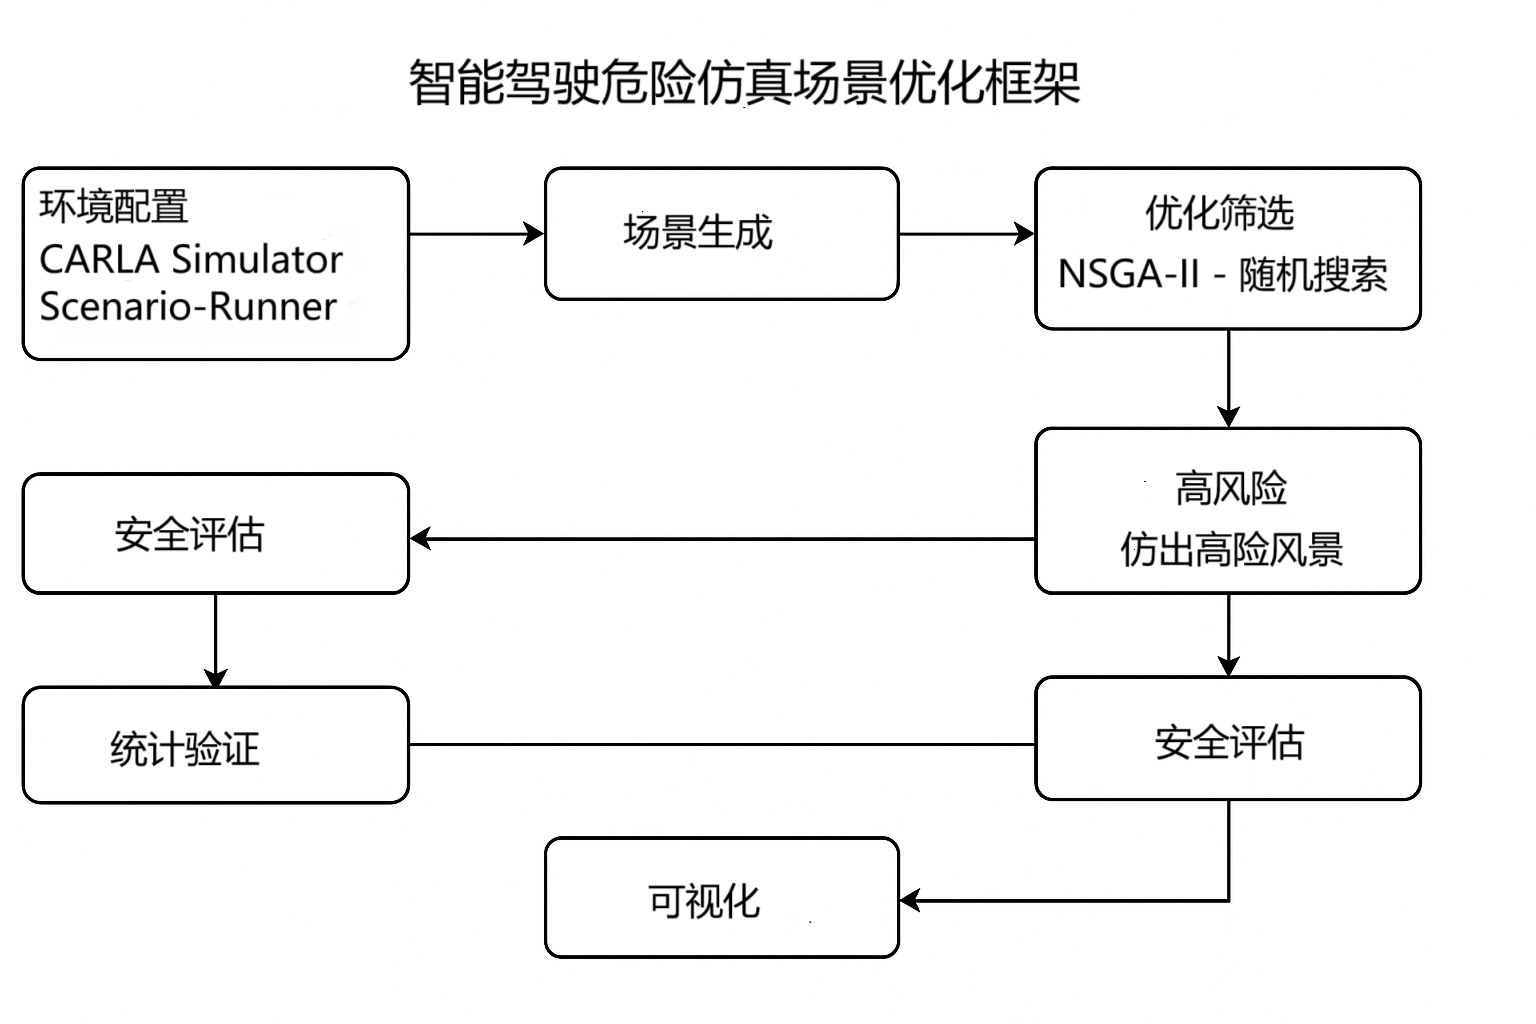
\includegraphics[width=0.8\textwidth]{figure1.png} % 调整宽度为文本宽度的80%
	\caption{图1} % 自动编号(如"图1:")
	\label{fig:example} % 用于交叉引用
\end{figure}


智能体训练(train\_agent 模式):对在第一阶段选出的对抗性场景进行RL训练。调用示例如下:

python scripts/run\_train.py --agent\_cfg=adv\_scenic.yaml --scenario\_cfg=train\_agent\_scenic.yaml --mode train\_agent --scenario\_id 1

此处使用与场景选择阶段同样的adv\_scenic.yaml配置文件,以及train\_agent\_scenic.yaml场景配置(包含从第一阶段得到的最难场景信息)。训练过程中,使用前8条固定路线进行训练(其余2条用于测试),以提高智能体在这些高风险场景下的表现。


\begin{figure}[htbp]
	\centering
	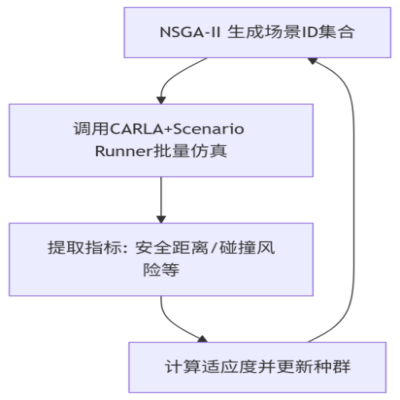
\includegraphics[width=0.8\textwidth]{figure2.png} % 调整宽度为文本宽度的80%
	\caption{图2} % 自动编号(如"图1:")
	\label{fig:example} % 用于交叉引用
\end{figure}



评估模式(eval 模式):在训练后,对训练好的智能体进行测试评估。调用示例如下:

python scripts/run\_eval.py --agent\_cfg=adv\_scenic.yaml --scenario\_cfg=eval\_scenic.yaml --mode eval --scenario\_id 1 --test\_epoch -1

其中eval\_scenic.yaml定义了评估场景(通常为与训练不同的路线),test\_epoch指定加载的模型检查点(-1表示使用最终训练模型)。评估过程中统计碰撞、路线完成等指标。



\begin{figure}[htbp]
	\centering
	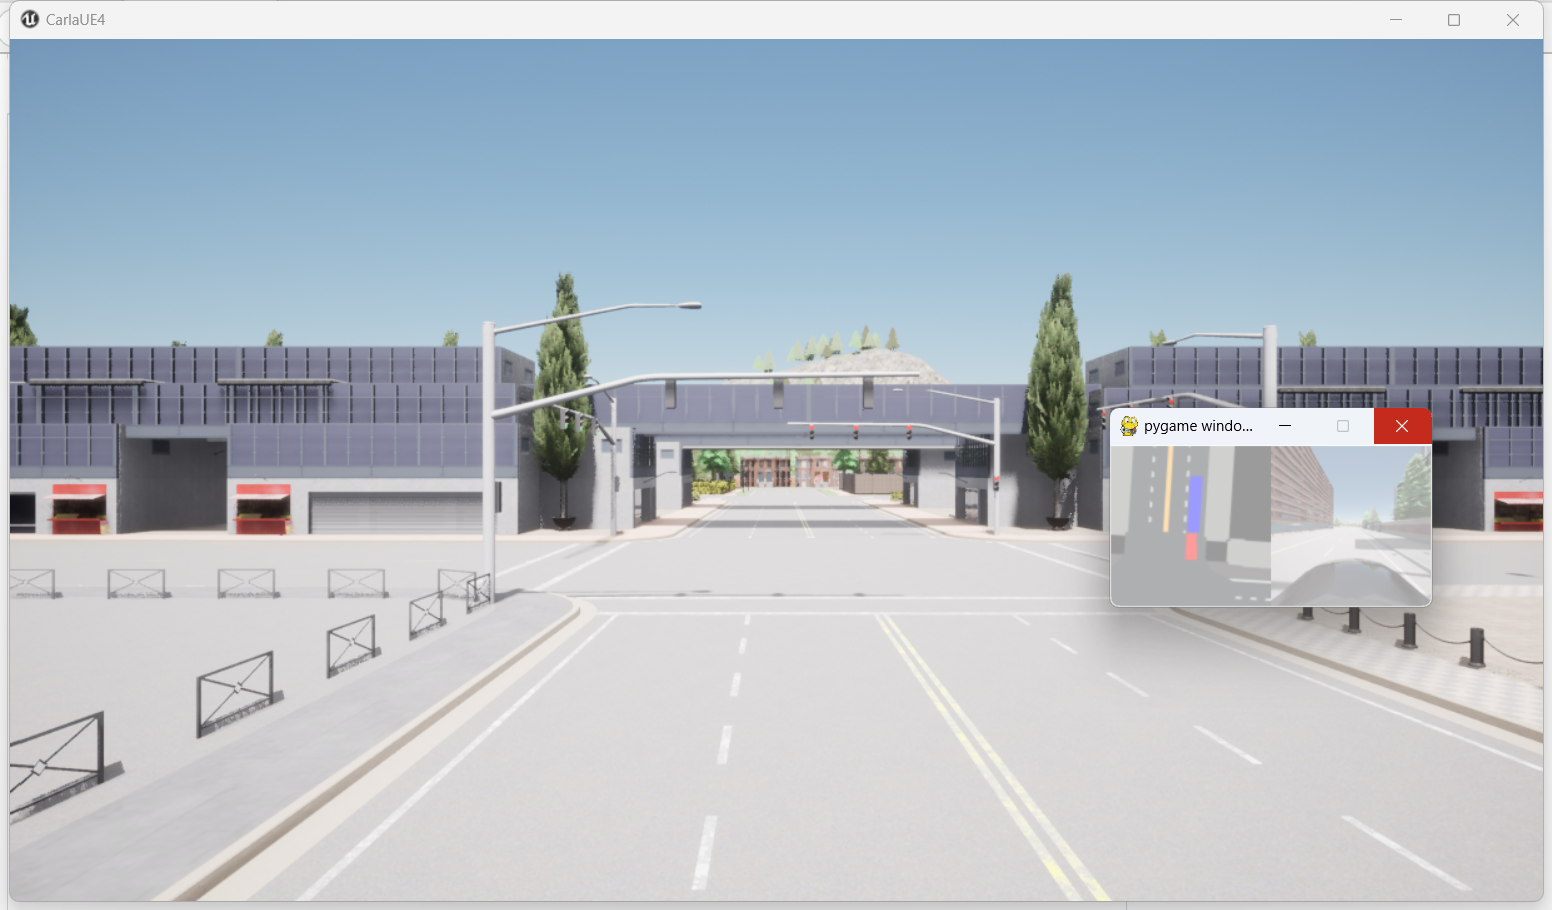
\includegraphics[width=0.8\textwidth]{figure3.png} % 调整宽度为文本宽度的80%
	\caption{图3} % 自动编号(如"图1:")
	\label{fig:example} % 用于交叉引用
\end{figure}



动态语言驱动场景(dynamic 模式):首先将自然语言描述转录到retrieve/scenario\_descriptions.txt,运行python retrieve.py,生成对应的Scenic场景脚本文件。然后使用run\_train\_dynamic.py脚本启动场景优化或训练,例如:

python scripts/run\_train\_dynamic.py --agent\_cfg=adv\_scenic.yaml --scenario\_cfg=dynamic\_scenic.yaml --mode train\_scenario

这里dynamic\_scenic.yaml用于指定动态生成场景的配置,脚本会在线检索或调用LLM生成新的场景并进行训练。


\begin{figure}[htbp]
	\centering
	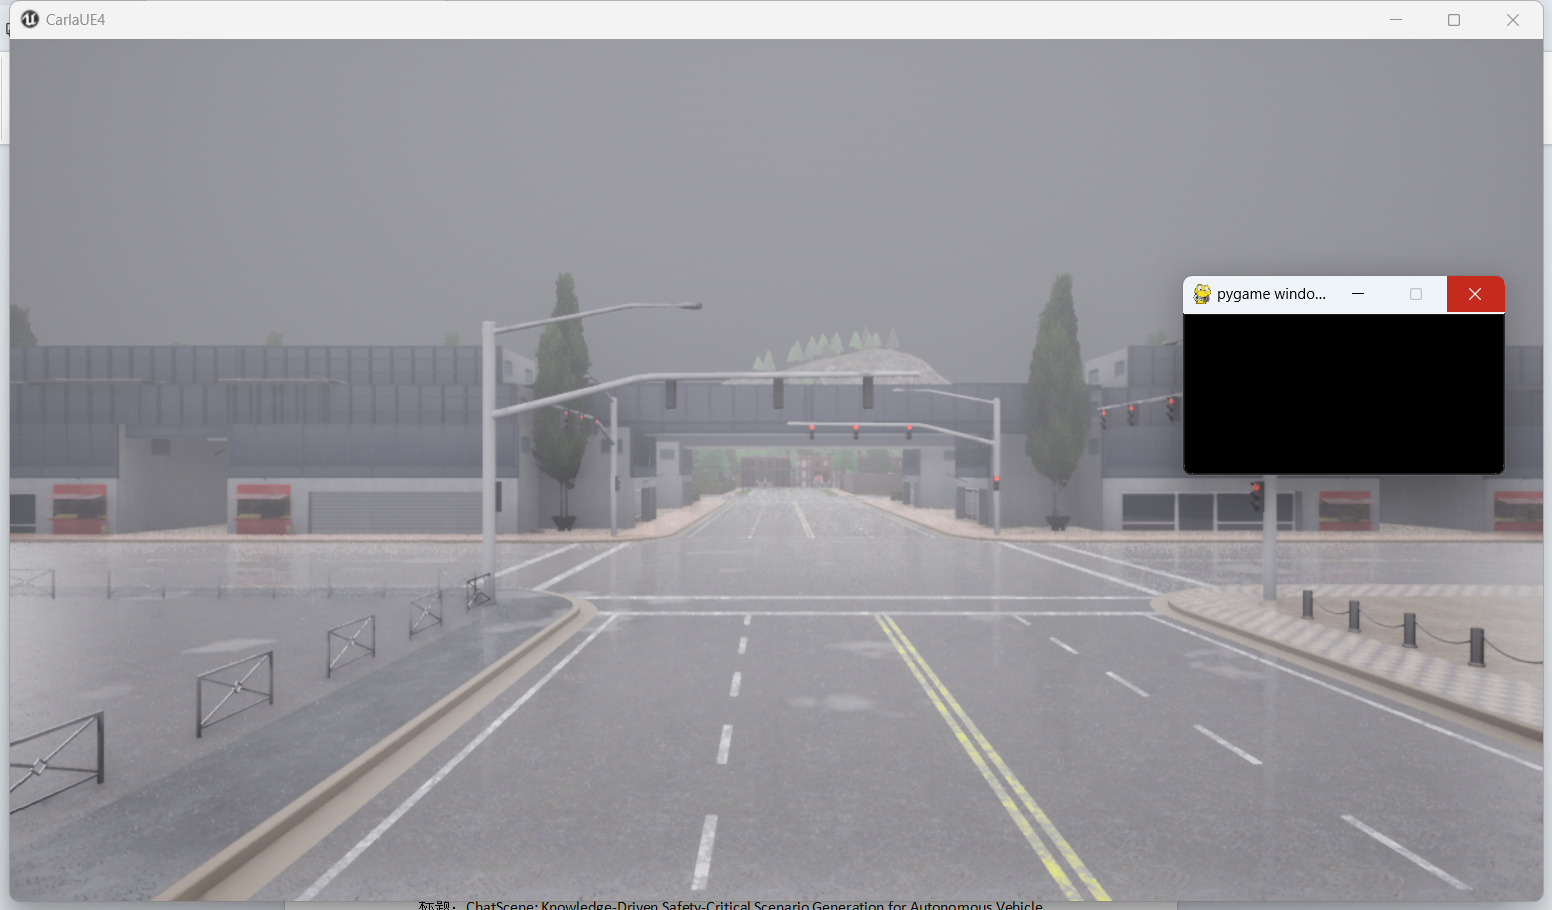
\includegraphics[width=0.8\textwidth]{figure4.png} % 调整宽度为文本宽度的80%
	\caption{图4} % 自动编号(如"图1:")
	\label{fig:example} % 用于交叉引用
\end{figure}




\section{ASIL-Gen 场景优化与分类}
场景生成

基于基础场景模板,通过脚本自动化生成 13 类场景变体,包括动态障碍物交叉、无信号路口冲突、恶劣天气下的跟车等复杂情况。每个变体通过调整障碍物位置、速度、交通流量等参数,形成多样化的测试场景,全面覆盖自动驾驶系统可能面临的风险工况。

优化算法

NSGA-II:以碰撞概率与场景复杂度作为双目标函数。碰撞概率通过预测车辆、行人等交通参与者的运动轨迹计算;场景复杂度则综合考虑交通参与者数量、道路拓扑结构、环境干扰因素等指标。利用 NSGA-II 算法搜索帕累托前沿,筛选出既具有高风险价值又具备代表性的场景。​
随机搜索:随机生成场景参数组合作为基线方法,通过对比 NSGA-II 算法与随机搜索在目标函数上的表现,验证 NSGA-II 在场景优化方面的优越性。

ASIL 分类

依据 ISO 26262 标准,基于暴露频率(Exposure)、可控性(Controllability)与严重性(Severity)三个维度,构建量化评估模型计算安全等级。通过专家打分与数据统计相结合的方式,确定各维度权重,将场景划分为 ASIL-A、ASIL-B、ASIL-C、ASIL-D 四个安全等级,为自动驾驶系统的风险评估提供标准化依据。


\section{讨论与未来工作}
\subsection{优势与局限}

优势:

ChatScene 与 ASIL-Gen 的协同架构为自动驾驶测试带来了显著革新。ChatScene 凭借自然语言驱动的动态场景生成与基于强化学习的固定场景优化,打破了传统场景生成的模式限制。在动态模式下,用户可通过简单的自然语言描述,快速获取多样化的复杂场景,如 “冰雪路面上,校车突然开门,后方电动车紧急避让”,这种灵活性极大提升了测试场景的构建效率;固定场景模式则通过 SAC 算法优化,精准模拟各类交通参与者行为,为自动驾驶系统提供标准化测试模板。ASIL-Gen 引入 NSGA-II 多目标优化算法与量化评估模型,以碰撞概率、场景复杂度等为核心指标,科学筛选高风险场景,将 ASIL-D 等级场景占比提升至 15\%,相比传统随机搜索方法,大幅提高了测试的针对性与有效性。二者结合,不仅覆盖了从简单到极端的广泛场景,还实现了从场景生成到安全评估的闭环,显著提升了自动驾驶测试的覆盖率与深度。


局限:

尽管取得诸多突破,当前方案仍存在明显局限性。ChatScene 的动态模式高度依赖 GPT-4o 的生成能力,在实际应用中,语言模型可能产生逻辑错误或与交通规则不符的场景代码。例如,生成 “车辆在双黄实线处掉头且无任何警示” 的不合理场景,此类错误会导致测试结果的可信度降低。此外,由于 GPT-4o 的调用成本较高且存在响应延迟,限制了大规模实时测试的开展。同时,ASIL-Gen 的评估标准主要基于现有交通规则与静态场景参数,对新兴的交通场景(如车路协同环境下的交互场景)以及动态交通流变化的评估能力不足,难以全面反映自动驾驶系统在复杂现实环境中的安全风险。

\subsection{未来方向}
融合多模态输入,增强场景真实性

为使生成场景更贴近真实驾驶环境,未来将深度融合激光雷达、摄像头、毫米波雷达及高精地图等多模态数据。通过多传感器数据的时空对齐与特征融合,构建高精度的三维场景模型。例如,利用激光雷达获取精确的目标距离与形状信息,结合摄像头的纹理与色彩数据,可更真实地还原道路障碍物、行人等目标;毫米波雷达在恶劣天气下的稳定探测能力,能有效弥补其他传感器的不足。同时,将高精地图中的道路拓扑结构、交通标志语义等信息融入场景生成过程,使生成场景不仅在物理形态上逼真,还能准确反映交通规则约束,为自动驾驶系统提供更具挑战性与真实性的测试环境。



扩展 ASIL 分类标准,纳入高德 MapDR 驾驶规则

目前的 ASIL 分类标准在语义理解与规则覆盖上存在局限性,未来将深度整合高德 MapDR 的驾驶规则语义,实现评估体系的全面升级。​
规则语义解析与融合:高德 MapDR 数据包含丰富的交通规则语义信息,如特定路段的限速变化、路口的优先通行权规则、特殊区域的驾驶限制等。通过自然语言处理与知识图谱技术,提取 MapDR 数据中的规则语义,并将其转化为可量化的评估指标。例如,将 “学校区域限速 30km/h” 规则转化为场景中车辆速度的约束条件,若自动驾驶车辆在该区域超速行驶,则相应提升场景的安全风险等级。​
动态风险评估模型构建:结合 MapDR 的实时交通信息(如拥堵状态、事故预警),构建动态的 ASIL 评估模型。在交通拥堵场景下,根据 MapDR 提供的车流密度、平均车速等数据,动态调整碰撞概率与可控性评估权重,使安全等级评估更贴合实际风险状况。同时,将 MapDR 中的驾驶习惯数据(如不同地区的跟车距离偏好、变道频率)纳入评估,更准确地模拟人类驾驶行为对自动驾驶系统的影响。​
跨场景规则泛化应用:基于 MapDR 的海量场景数据,训练规则泛化模型,使 ASIL 分类标准能够适应不同地域、不同交通环境下的规则差异。通过迁移学习与强化学习算法,让评估模型在新场景中快速识别并应用相应的交通规则,提高 ASIL 分类的普适性与准确性,为自动驾驶系统在复杂多变的现实交通环境中的安全评估提供更可靠的依据。

\newpage


